\documentclass[a4paper]{article}

\usepackage{graphicx}
\usepackage{amsmath}
\usepackage{hyperref}
\usepackage{geometry}
\usepackage{listings}
\usepackage{color}


\definecolor{dkgreen}{rgb}{0,0.6,0}
\definecolor{gray}{rgb}{0.5,0.5,0.5}
\definecolor{mauve}{rgb}{0.58,0,0.82}

\title{َ\textbf{ANS Research Assignment 2}}
\author{ Professor Sayad\\ Amirhossein Moradian\\  810100467}

\lstset{frame=tb,
	language=Java,
	aboveskip=3mm,
	belowskip=3mm,
	showstringspaces=false,
	columns=flexible,
	basicstyle={\small\ttfamily},
	numbers=none,
	numberstyle=\tiny\color{gray},
	keywordstyle=\color{blue},
	commentstyle=\color{dkgreen},
	stringstyle=\color{mauve},
	breaklines=true,
	breakatwhitespace=true,
	tabsize=3
}

\begin{document}
	
	\begin{figure}
		\centering
		
\includegraphics[scale=0.75]{Figures/UT1}
	\end{figure}
	
	\maketitle
	
	\section*{Introduction}	
	In the following report, four plots are given on separate pages. First plot goes to finding the average $I(t)$ for the 50 experiments and plotting it. Second one goes to Tang et al's article. Third one goes to De et al's article. and finally the last goes to plotting all the curves into one plot for comparison.
	\pagebreak
	
	\section{Finding the average $I(t)$ for the 50 experiments plot}
	\begin{figure}[h]
		\centering
		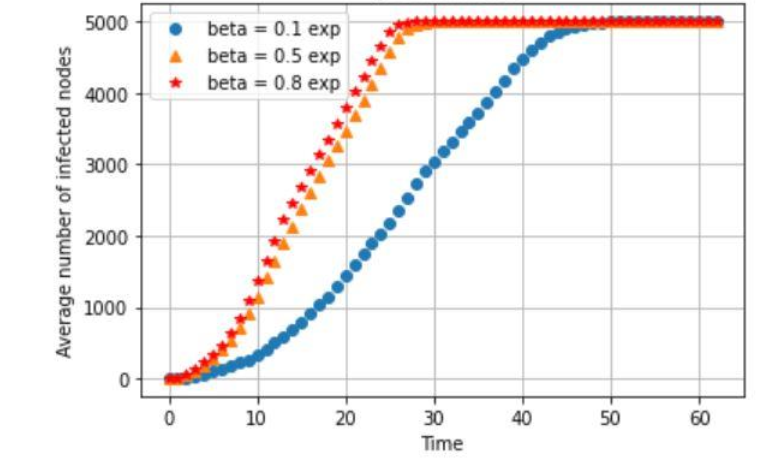
\includegraphics[scale=0.6]{Figures/Fig1}
	\end{figure}
	\pagebreak
	
	\section{Tang et al's model Plot}
	\begin{figure}[h]
		\centering
		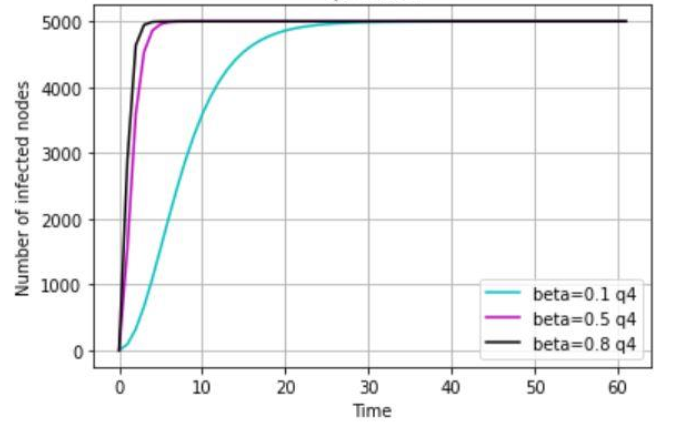
\includegraphics[scale=0.6]{Figures/Fig2}
	\end{figure}
	\pagebreak
	
	\section{De et al's model Plot}
	\begin{figure}[h]
		\centering
		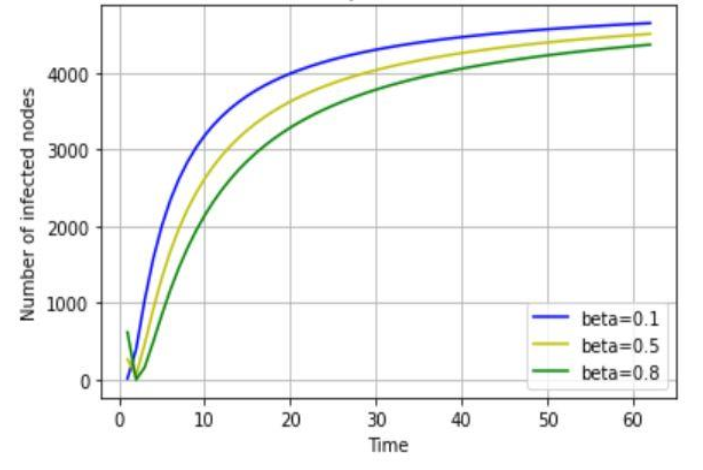
\includegraphics[scale=0.6]{Figures/Fig3}
	\end{figure}
	\pagebreak
	
	\section{Comparison Plot}
	\begin{figure}[h]
		\centering
		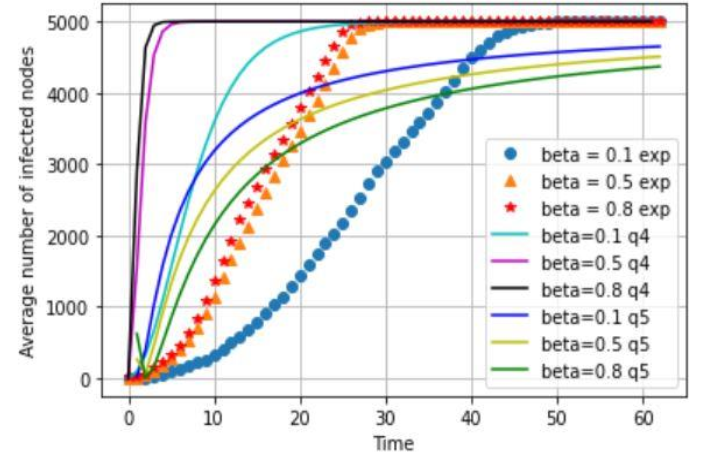
\includegraphics[scale=0.6]{Figures/Fig4}
	\end{figure}
	\pagebreak
	
\end{document}